\chapter{Tensor Networks}

\section{Matrix Product States}
\subsection{Finite-dimensional lattices}

    \newdef{Matrix product state}{\index{MPS}
        Let $\mathcal{H}_n$ be the local Hilbert spaces of dimension $d_n$ where $n\in\{1,\ldots,N\}$. A state $|\psi\rangle$ in the total Hilbert space $\bigotimes_i\mathcal{H}_i$ is a matrix product state (with periodic boundary conditions) if there exist matrices $A^{i_n}(n)\in\mathcal{L}(\mathbb{C}^{D_n}, \mathbb{C}^{D_{n-1}})$ with $i_n\leq d_n$ such that
        \begin{gather}
            |\psi\rangle = \sum_{\{i_k\}}\text{tr}\Big(\prod_n^NA^{i_n}(n)\Big)|i_1\ldots i_N\rangle.
        \end{gather}
        For each lattice site $n$ the set of matrices $\{A^{i_n}_{\alpha\beta}(n)\}$ can be regarded as the content of one rank-3 tensor. The periodic boundary condition requires that $D_0=D_N$ (otherwise the trace would be ill-defined). Different boundary conditions can be implemented by inserting an additional factor $X$ at the end of the trace.
    }
    \begin{notation}
        In the continuation of this chapter we will abbreviate matrix product states as \textbf{MPS}.
    \end{notation}

    \begin{remark}[Physical and virtual spaces]
        For each \textit{physical} index $i_n$ one can regard the matrix $A^{i_n}(n)$ as a linear map between \textit{virtual} (or ancilla) spaces $\mathbb{C}^{D_n}$.
    \end{remark}

    \newformula{MPS projector}{
        Consider an MPS given by tensors $\{A(n)\}_{n\leq N}$. The associated MPS projector is defined as:
        \begin{gather}
            \mathcal{P}(A) = \sum_{i, \alpha, \beta}A^i_{\alpha\beta}(n)|i\rangle\langle\alpha\beta|
        \end{gather}
    }

    \newformula{Transfer operator}{\index{transfer!operator}
        Give the MPS tensors $\{A(n)\}_{n\leq N}$ one can define a transfer operator:
        \begin{gather}
            \label{tennet:transfer_operator}
            \mathbb{E}(n) = \sum_{i=1}^{d_n}A^i(n)\otimes\overline{A^i}(n)
        \end{gather}
    }
    \begin{formula}[Superoperator]\index{super!operator}
        More generally we can define for every local observable $\hat{O}_n$ a superoperator in $\mathcal{L}(\mathbb{C}^{D_n}\otimes\overline{\mathbb{C}^{D_n}}, \mathbb{C}^{D_{n-1}}\otimes\overline{\mathbb{C}^{D_{n-1}}})$:
        \begin{gather}
            \mathbb{E}_{O_n}(n) = \sum_{i,i'=1}^{d_n}\langle i|\hat{O}_n|i' \rangle A^{i'}(n)\otimes\overline{A^i}(n)
        \end{gather}
        Comparing with the definition of the transfer operator we see that $\mathbb{E}$ is given by the superoperator associated to the unit operator. Given two sets of MPS tensors $\{A(n)\}, \{B(n)\}$ we define a generalized superoperator by:
        \begin{gather}
            \mathbb{E}^A_B(n) = \sum_{i=1}^{d_n}A^i(n)\otimes\overline{B^i}(n)
        \end{gather}
    \end{formula}
    \begin{example}
        Using these definitions we can rewrite the formulas for expectation values more efficiently. Given a product operator $\hat{O}=\bigotimes_i^N\hat{O}_i$ we find that:
        \begin{gather}
            \langle\psi[A]|\hat{O}|\psi[A]\rangle = \text{tr}\Big(\mathbb{E}_{O_1}(1)\cdots\mathbb{E}_{O_N}(N)\Big)
        \end{gather}
    \end{example}

    \begin{formula}
        Associated to the superoperator $\mathbb{E}_O(n)$ one can define a map acting on the virtual operators:
        \begin{align}
            \mathcal{E}^{(n)}_{O_n}(\phi) &= \sum_{i, i'=1}^{d_n}\langle s|\hat{O}_n|s' \rangle A^{i'}(n)\phi A^i(n)^\dag\\
            \tilde{\mathcal{E}}^{(n)}_{O_n}(\phi) &= \sum_{i, i'=1}^{d_n}\langle s|\hat{O}_n|s' \rangle A^i(n)^\dag\sigma A^{i'}(n)
        \end{align}
        where $\phi\in\mathcal{L}(\mathbb{C}^{D_n}), \sigma\in\mathcal{L}(\mathbb{C}^{D_{n-1}})$.
    \end{formula}
    \begin{property}
        The map $\mathcal{E}_{\mathbbm{1}}^{(n)}$ associated to the transfer operator is a CP map\footnote{See definition \ref{operator:cp_map}.} and the associated Kraus operators are the MPS matrices $A^i(n)$.
    \end{property}

\subsection{Injectivity}\index{injective!MPS}

    For translation-invariant MPS one can use an easier definition:
    \newadef{Injective MPS}{
        A translation-invariant MPS is said to be injective if its transfer operator has a unique maximal eigenvalue.
    }

    In the next sections we will always assume the MPS to be injective unless stated otherwise.

\subsection{Gauge freedom and canonical forms}

    \begin{property}[Gauge freedom]
        As is clear from the construction of matrix product states there exists some freedom in the representation of the MPS tensors. One can always perform a transformation of the form $A(n)\rightarrow X^{-1}(n)A(n)X(n+1)$.
    \end{property}
    \begin{remark}
        If we use periodic boundary conditions then we must require that $X(L+1)=X(1)$ where $L$ is the lattice size.
    \end{remark}

    Using the gauge freedom in the representation of a generic MPS one can construct certain forms which have useful properties:
    \begin{construct}[Left canonical form\footnotemark]
        \footnotetext{Also called the \textbf{left isometric form}, \textbf{left orthogonal form} or just \textbf{left gauge}.}
        This form is specified by the following property:
        \begin{gather}
            \begin{tikzpicture}
                \node[rectangle,draw=black,minimum size=20] (A) at (0,1) {$A_L$};
                \node[rectangle,draw=black,minimum size=20] (Ad) at (0,-1) {$\overline{A_L}$};
                \draw (A) -- (Ad);
                \draw (A) to[out=200,in=160] (Ad);
                \draw (A) -- +(1,0);
                \draw (Ad) -- +(1,0);
                \node (E) at (1.5,0) {$=$};
                \node (A2) at (3,1) {};
                \node (Ad2) at (3,-1) {};
                \draw (A2) to[out=200,in=160] (Ad2);
            \end{tikzpicture}
        \end{gather}
        Any MPS can be brought in this form. First we construct the transfer operator $\mathbb{E}(n)$ for every site and find its maximal eigenvector. By the \textit{Perron-Frobenius theorem} this eigenvector (which is in fact a matrix itself) is positive and hence allows a decomposition of the form $\lambda(n)=L^\dag(n)L(n)$. The left orthogonal forms are then defined by
        \begin{gather}
            A_L(n) = L(n)A(n)L^{-1}(n+1)
        \end{gather}
    \end{construct}
    \sremark{In a similar manner one can construct the right orthogonal form $A_R$.}

    \begin{method}[Vidal]\index{Vidal}
        Given a general quantum state in terms of an $n$-leg tensor there exists an efficient way of constructing the left (or right) canonical forms introduced by Vidal \cite{VidalCanForm}. For this we perform a cut between the first and second site and apply a singular value decomposition to obtain a tensor of the form $U^{[1]}SV^{[2, ...]}$. One can now recursively apply this procedure to the product of the singular values $S$ and the right unitary $V$.
    \end{method}

    \begin{construct}[Mixed canonical form]
        We can combine the left and right canonical forms. Let $L(n)$ and $R(n)$ be the decompositions of the left and right eigenvectors of the transfer operator at site $n$, i.e. $\lambda(n)=L^\dag(n)L(n)$ and $\rho(n)=R(n)R^\dag(n)$. The left and right canonical forms are then related by a matrix $C(n)$ in the following way: $A_L(n)C(n+1)=C(n)A_R(n)$. These matrices are given by
        \begin{gather}
            C(n)=L(n)R(n)
        \end{gather}
    \end{construct}

\subsection{Translation-invariant states}

    \newdef{Uniform MPS}{
        By setting all MPS tensors $A(n) = B$ for a given tensor $B$ one obtains a translation-invariant (TI) state, i.e. a state invariant under a shift of the index $n$. These MPS form the variational class of uniform MPS.
    }
    \begin{remark}[TIMPS]
        Not every TIMPS is uniform, there should only exist a local gauge transformation $A'(n) = U(n-1)A(n)U(n)^{-1}$ such that $A'(n)$ is uniform (in certain cases this is only possible by enlarging the bond dimension).
    \end{remark}

\section{Matrix product operators}

    \newdef{Matrix product operator\footnotemark}{\index{MPO}
        \footnotetext{As in the case of matrix product states we will abbreviate this as \textbf{MPO}.}
        Starting from the general form of an MPS one can easily construct more general objects. By replacing the rank-3 tensors $A^i(n)$ with rank-4 tensors $A^{i,j}(n)$ and $|i_1\cdots i_n\rangle$ by $|i_1\rangle\langle j_1|\otimes\cdots\otimes|i_n\rangle\langle j_n|$ one obtains the notion of a matrix product operator:
        \begin{gather}
            \hat{O} = \sum_{\{i_k,j_l\}}\text{tr}\Big(\prod_{m,n=1}^NO^{i_m,j_n}(n)\Big)|i_1\cdots i_N\rangle\langle j_1\cdots j_n|
        \end{gather}
        or in terms of a basis $\{\hat{O}_i\}$ for the space of local operators:
        \begin{gather}
            \hat{O} = \sum_{\{i_k\}}\text{tr}\Big(\prod_n^NA^{i_n}(n)\Big)\hat{O}_{i_n}
        \end{gather}
    }

    \begin{method}[Local Hamiltonian to MPO]
        Given a local Hamiltonian $\hat{H}=\sum_i\hat{H}^{(i)}$ one can build an MPO which generates this Hamiltonian\footnote{In fact one can use this procedure to turn any local operator into an MPO.}:
        \begin{gather}
            \hat{H} = \sum_{\{i_k,j_l\}}\text{tr}\Big(\prod_{m,n=1}^NA^{i_m,j_n}(n)\Big)|i_1\cdots i_N\rangle\langle j_1\cdots j_n|
        \end{gather}
        To obtain this MPO form one uses the concept of a cellular automaton. This is a set of possible states together with a set of rules that tell you how you can go from one state to another. To obtain the set of states in our case we look at a given site $i$. All distinct combinations of 1-site operators to the right of $i$ give rise to a distinct state $\mu$. The transition rules are obtained by looking at which operator can be placed at the site $i$ in a way consistent with the form of the given Hamiltonian.
    \end{method}
    \begin{example}
        Consider a 2-site Hamiltonian of the form \[\hat{A}\otimes\hat{B}\otimes\mathbbm{1}\otimes\cdots+\mathbbm{1}\otimes\hat{A}\otimes\hat{B}\otimes\mathbbm{1}\otimes\cdots+\cdots\] Looking at a specific site $i$ we obtain 3 distinct possibilities:
        \begin{enumerate}
            \item We have only identity operators acting to the right of $i$.
            \item Immediately to the right we have the operator $\hat{B}$ acting on $i+1$.
            \item Somewhere to the right we find the combination $\hat{A}\otimes\hat{B}$.
        \end{enumerate}
        The transition rules for this automaton are then given by the following list:
        \begin{itemize}
            \item $1\rightarrow2$: $\mathbbm{1}$
            \item $1\rightarrow2$: $\hat{B}$
            \item $2\rightarrow3$: $\hat{A}$
            \item $3\rightarrow3$: $\mathbbm{1}$
        \end{itemize}
        What is useful for us is that this set of transition rules can be turned into a matrix: \[T=\begin{pmatrix}\mathbbm{1}&\hat{B}&0\\0&0&\hat{A}\\0&0&\mathbbm{1}\end{pmatrix}\] The MPO is then obtained by setting the MPO matrix $A$ equal to $T$ at every site.
    \end{example}

\subsection{MPO-injectivity}

    The main reference for this section is \cite{sahinoglu_mpo}.

    \newdef{MPO-injective PEPS}{\index{MPO!injectivity}
        Consider a trivalent PEPS network on a manifold $M$ and select a simply-connected subregion $\Omega\subset\Lambda$. By contracting the tensors withing this region one obtains a linear map \[A_\Lambda:(\mathbb{C}^D)^{\otimes|\Lambda|}\rightarrow(\mathbb{C}^d)^{\otimes|\partial\Lambda|}\] from the virtual spaces on the edges to the physical space living in the bulk. This PEPS is said to be MPO-injective if there exists a linear map (four-leg tensor) \[M:\mathbb{C}^D\otimes\mathbb{C}^m\rightarrow \mathbb{C}^D\otimes\mathbb{C}^m\] such that for every subregion $\Omega\subset\Lambda$ the linear map $A_\Lambda$ is injective on a (maximal) subspace $S$ for which the projector onto $S$ can be written as an MPO constructed from the tensors $M$ living on the boundary $\partial\Lambda$. (See figure \ref{tennet:fig:mpo_injectivity}: the tensors $M$ are given by crossings of black and red lines.)
        \begin{figure}[ht!]
            \centering
            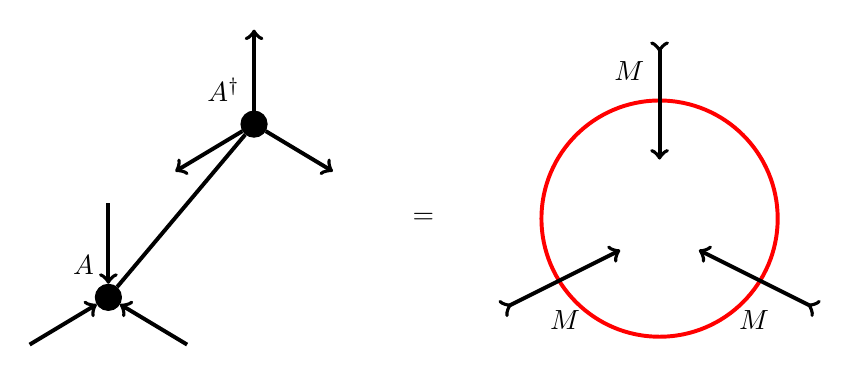
\begin{tikzpicture}
                \node[circle,draw=black,fill=black,minimum size=5pt,label={110:$A$}] (T) at (0,-1) {};
                \node[circle,draw=black,fill=black,minimum size=5pt,label={110:$A^\dag$}] (T2) at (1.85,1.2) {};
                \node (E) at (4,0) {$=$};
                \node[label={120:$M$}] (M1) at (7, 1.5) {};
                \node[label={-90:$M$}] (M2) at (8.2, -0.92) {};
                \node[label={-90:$M$}] (M3) at (5.8, -0.92) {};
                \draw[line width=0.5 mm] (T) -- (T2);
                \draw[<-, line width=0.5 mm] (T) -- +(0,1.2);
                \draw[<-, line width=0.5 mm] (T) -- (1, -1.6);
                \draw[<-, line width=0.5 mm] (T) -- (-1, -1.6);
                \draw[->, line width=0.5 mm] (T2) -- +(0,1.2);
                \draw[->, line width=0.5 mm] (T2) -- (2.85, 0.6);
                \draw[->, line width=0.5 mm] (T2) -- (0.85, 0.6);
                \draw[draw=red, line width=0.5 mm] (7, 0) circle (1.5);
                \draw[<-<, line width=0.5 mm] (7, 0.75) -- (7, 2.25);
                \draw[<-<, line width=0.5 mm] (7.5, -0.4) -- (9, -1.15);
                \draw[<-<, line width=0.5 mm] (6.5, -0.4) -- (5, -1.15);
            \end{tikzpicture}
            \caption{MPO-injective PEPS.}
            \label{tennet:fig:mpo_injectivity}
        \end{figure}
    }

    \begin{axiom}[Pulling-through]\index{pulling-through condition}
        One of the key features of topological order is that this cannot be detected locally, only a global measurement can show the existence of topologically ordered states. To this end we introduce an axiom such that one can pull an MPO through the lattice. Graphically this is shown in figure \ref{tennet:fig:pulling_through}.
        \begin{figure}[ht!]
            \centering
            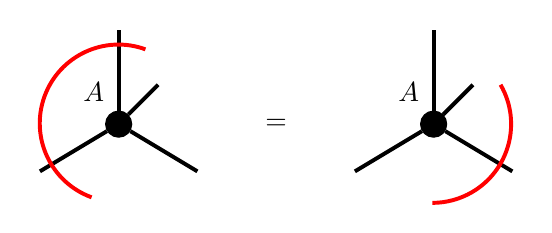
\begin{tikzpicture}
                \node[circle,draw=black,fill=black,minimum size=5pt,label={110:$A$}] (T) at (0,0) {};
                \node[circle,draw=black,fill=black,minimum size=5pt,label={110:$A$}] (T2) at (4,0) {};
                \node (E) at (2,0) {$=$};
                \draw[line width=0.5 mm] (T) -- +(0.5,0.5);
                \draw[line width=0.5 mm] (T) -- +(0,1.2);
                \draw[line width=0.5 mm] (T) -- (1, -0.6);
                \draw[line width=0.5 mm] (T) -- (-1, -0.6);
                \draw[line width=0.5 mm, draw=red] (0.34, 0.95) arc (70:250:1);
                \draw[line width=0.5 mm] (T2) -- +(0.5,0.5);
                \draw[line width=0.5 mm] (T2) -- +(0,1.2);
                \draw[line width=0.5 mm] (T2) -- (5, -0.6);
                \draw[line width=0.5 mm] (T2) -- (3, -0.6);
                \draw[line width=0.5 mm, draw=red] (4.85, 0.5) arc (30:-90:1);
            \end{tikzpicture}
            \caption{Pulling-through condition.}
            \label{tennet:fig:pulling_through}
        \end{figure}
    \end{axiom}

\subsection{MPO-symmetries for SPT phases}

    One can generalize the above framework to include not only pure topological order but also symmetry-protected topological order (see reference \cite{bultinck_mpo}). For this one has to slightly modify the axioms from the last section:
    \begin{axiom}[Pulling-through for SPT phases]\index{pulling-through condition}
        When pulling a symmetry-MPO through a tensor one has to act with a unitary on the physical level. Graphically this is shown in figure \ref{tennet:fig:pulling_through_spt}.
        \begin{figure}[ht!]
            \centering
            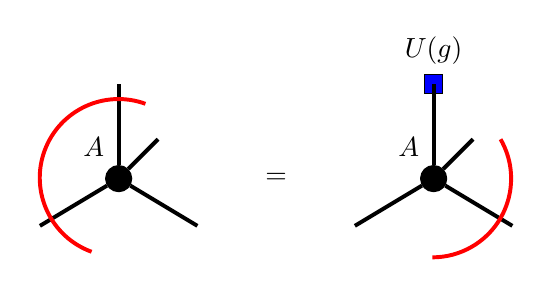
\begin{tikzpicture}
                \node[circle,draw=black,fill=black,minimum size=5pt,label={110:$A$}] (T) at (0,0) {};
                \node[circle,draw=black,fill=black,minimum size=5pt,label={110:$A$}] (T2) at (4,0) {};
                \node[rectangle, draw=black, fill=blue, minimum size=2pt, label={$U(g)$}] (U) at (4, 1.2) {};
                \node (E) at (2,0) {$=$};
                \draw[line width=0.5 mm] (T) -- +(0.5,0.5);
                \draw[line width=0.5 mm] (T) -- +(0,1.2);
                \draw[line width=0.5 mm] (T) -- (1, -0.6);
                \draw[line width=0.5 mm] (T) -- (-1, -0.6);
                \draw[line width=0.5 mm, draw=red] (0.34, 0.95) arc (70:250:1);
                \draw[line width=0.5 mm] (T2) -- +(0.5,0.5);
                \draw[line width=0.5 mm] (T2) -- +(0,1.2);
                \draw[line width=0.5 mm] (T2) -- (5, -0.6);
                \draw[line width=0.5 mm] (T2) -- (3, -0.6);
                \draw[line width=0.5 mm, draw=red] (4.85, 0.5) arc (30:-90:1);
            \end{tikzpicture}
            \caption{Pulling-through condition for SPT phases.}
            \label{tennet:fig:pulling_through_spt}
        \end{figure}
    \end{axiom}